\documentclass[11pt]{article}
\usepackage[paper=letterpaper,margin=2cm]{geometry}
\usepackage{amsmath}
\usepackage{amssymb}
\usepackage{amsfonts}
\usepackage{newtxtext, newtxmath}
\usepackage{titling}
\usepackage{graphicx}
\usepackage[colorlinks=true]{hyperref}
\usepackage{listings}
\usepackage{caption}
\usepackage{subcaption}
\usepackage[section]{placeins}
\setlength{\droptitle}{-6em}

% Enter the specific assignment number and topic of that assignment below, and replace "Your Name" with your actual name.
\title{EE 585 Probabilistic Robotics: Assignment 1}
\author{Umut Kurt}
\date{\today}

\begin{document}
\maketitle
\section{Review and Use of a Robot Simulator}
\subsection{Ability to simulate the kinematics and/or dynamics of a differential drive (wheeled) robot}
    Before starting to simulate a differential drive robot, we should be familiar with some of the key concepts and terminology of the Webots. In Webots simulation environment, the different objects are called \textit{Nodes} and organized hierarchically in a \textit{Scene Tree}. A node may contain different sub-nodes, that can be set up by the user, corresponding to the characteristic of the node. For example \textit{Solid Nodes} are used to represent objects with physical properties such as dimension, mass and contact material. The solid class is the base class for collision-detected objects. Robot class is a subclass of the solid class.
    \\[\baselineskip]
    Webots offers a variety of off-the-shelf robot models that can be imported from \textit{PROTO nodes}. These robot models comes with built-in actuators, sensors and default controllers. Alternatively, a robot node can be used to built a differential drive robot model from scratch. Fundamental structure of the robot consists of two \emph{HingeJoint}, \emph{RotationalMotor} and \emph{PositionalSensor} nodes to simulate dynamics of a differential drive robot. In order to create a model of a differential robot, first a \emph{Robot} node is added. Then a \emph{Shape} node with box geometry is added to robot node, which is the body of the differential robot. The wheels of the robot are attached to the body by \emph{HingeJoint} nodes with cylindrical \emph{Solid} endpoints. \emph{HingeJoint} node offers three devices, in this case \emph{RotationalMotor} and \emph{PositionalSensor} will be used. For robot to stay in balance a caster wheel will be modeled. A caster wheel can be created by adding a ball joint with a \emph{Shape} node as a children. In the \emph{Shape} node, geometry is selected as sphere. Finally, \emph{Physics} node is very important for simulating a differential robot. If a robot contains a \emph{Physics} node, simulation will take into account the forces acting on solid bodies and the physical properties of these bodies. If the \emph{Physics} node is NULL, the motion will be simulated using kinematics mode which negates the forces that cause the motion and body will be treated as massless. The 3D model of the basic differential robot is shown in Figure \ref{fig:model}.
    
    \begin{figure}[ht!]
        \centering
        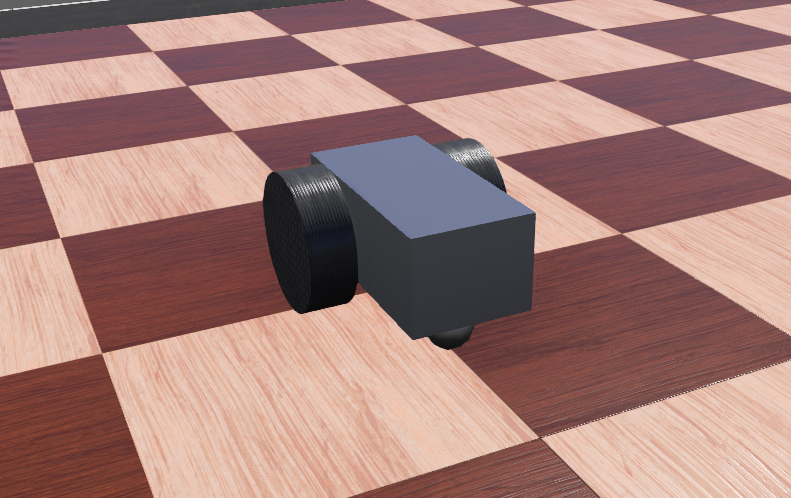
\includegraphics[width = 0.3\textwidth]{3d-model.PNG}
        \caption{3D model of the differential drive robot.}
        \label{fig:model}
    \end{figure}
    
    \subsection{Ability to command the linear and angular velocities of the robot}    
    In order to command the linear and angular velocities of the robot, a controller is required. A controller is a program that is executed by 
    the simulation engine at each time step. The actions of the robot is determined by the controller. In this assignment, controllers are written 
    in Python language.  Different controllers can be selected from the controller section inside the \emph{Robot} node.
    A linear velocity command can be given by setting the same velocities to both wheels. Linear velocity can be calculated by 
    multiplying the velocity and wheel radius. In the controller, first an 
    instance of the robot class is initialized. Then the \emph{RotationalMotor} devices are called using \emph{getDevice} method and enabled. The motors
    can be controlled eiter by setting the target velocity or by setting the target position using \emph{setVelocity} and \emph{setPosition} methods respectively.
    The example controller code is shown below. Further information about the controller can be found in \href{https://cyberbotics.com/doc/guide/controller-programming?tab-language=python}{the Webots documentation}.

    \begin{lstlisting}[language=Python]
        from controller import Robot, Motor
        # create the Robot instance.
        robot = Robot()
        # Initialize motors 
        motors = []
        motorNames = ['left_wheel', 'right_wheel']
        for i in range(len(motorNames)):
            motors.append(robot.getDevice(motorNames[i]))
            motors[i].setPosition(float('inf'))
            motors[i].setVelocity(0.0)
        # get the time step of the current world.
        timestep = int(robot.getBasicTimeStep())
        # Main loop:
        # - perform simulation steps until Webots is stopping the controller
        while robot.step(timestep) != -1:
            #set wheel velocity to 1 m/s
            for i in range(len(motorNames)):
                motors[i].setVelocity(1)   
            pass
    \end{lstlisting}

    During simulation, the linear velocity of the robot can be observed selecting robot. When the robot is selected four tabs appear below the \emph{Scene Tree} .
    Both linear and angular velocities of the robot in 3-axes can be observed in the \emph{Velocity} tab. Since wheel radius is $0.12 \ m$ and the commanded velocity is $1 \ m/s$ expected linear velocity is $0.12 \ m/s$. 
    The linear velocity of the robot is shown in Figure \ref{fig:linear}.

    \begin{figure}[ht!]
        \centering
        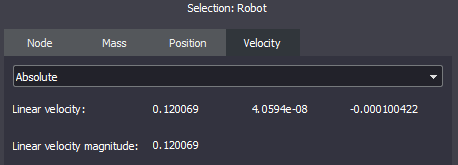
\includegraphics[width = 0.4\textwidth]{linear-velocity.PNG}
        \caption{Linear velocity of the robot.}
        \label{fig:linear}
    \end{figure}

    The angular velocity command can be given by setting different velocities to the wheels. As an example the left wheel is set to $1 \ m/s$ and the right wheel is set to $-1 \ m/s$. Robot turns around on the axis at the midpoint of the two differential wheels. The angular velocity of the robot can be calculated by dividing linear velocities of the wheels by the turning radius which is the half of the distance between wheels, in this case $0.18 \ m$. This corresponds to $\frac{0.12}{0.18} = 0.66 \ m/s$ The angular velocity of the robot is shown in Figure \ref{fig:angular}.

    \begin{figure}[ht!]
        \centering
        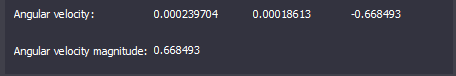
\includegraphics[width = 0.4\textwidth]{angular-velocity.PNG}
        \caption{Angular velocity of the robot.}
        \label{fig:angular}
    \end{figure}

    \subsection{Ability to simulate "real" noise into the motion kinematics/dynamics of the robot}

    In order to simulate "real" noise into the motion kinematics/dynamics of the robot, two different aprroaches applied together. First approach is to add random normal noise to velocity commands in the controller level. Second approach is to add \emph{ContactProperties} node for the wheels and modelling wheel slip. In order to model slip, the material of the wheels is stated and then in the \emph{WorldInfo} tab a \emph{ContactProperties} node is added for wheel material. The \emph{ContactProperties} node is used to define the friction coefficient between two materials. An assymetric coulomb friction is used to model slip. The friction coefficient is set to $0.4$. To illustrate the effect of slip, and the noise added to velocity command, the robot is commanded to move in a straight line for $0.3 \ m$.
    The simulation is run for $100$ times. The resulting positions of the robot is recorded using a GPS device and the output data is plotted in MATLAB. The results are shown in Figure \ref{fig:motion-noise}.
    \\ 

    \begin{figure}[ht!]
        \centering
        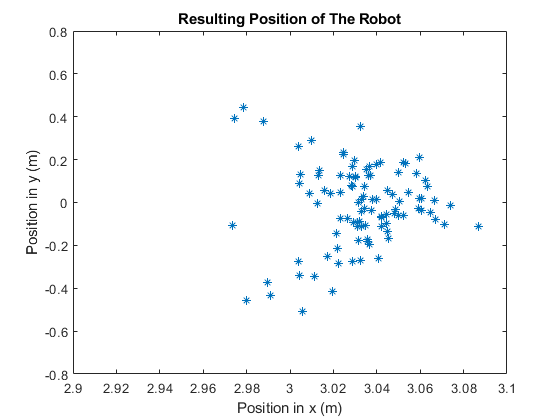
\includegraphics[width = 0.4\textwidth]{motion-noise.png}
        \caption{Motion noise.}
        \label{fig:motion-noise} 
    \end{figure}
 
    \subsection{Distance Sensor Data}
    As the distance sensor, a lidar 'Sick LMS 291' is used. Alternatively, a lidar node can be created from scratch. This device is added to the \emph{Robot} node, from \emph{PROTO nodes(Webots Projects)}, the sensor resolution is set to $180$ which corresponds to a precision of $1^{\circ}$ .
    In order to get the distance sensor data, sensor should be called using \emph{getDevice}, then enabled and finally the distance data can be obtained using \emph{getRangeImage} method.
    Data returns a list of distances, indexed by the angle of the corresponding sensor ray. The data is later saved to a csv file and plotted in MATLAB. The simulation environment and polar plot corresponding to the distance sensor data is shown in Figure \ref{fig:lidar}.
    Further information about the lidar sensor can be found in the \href{https://cyberbotics.com/doc/reference/lidar}{\emph{Webots Reference Manual} documentation}.
    
    \begin{figure}[ht!]
        \centering
        \begin{subfigure}[b]{0.3\textwidth}
            \centering
            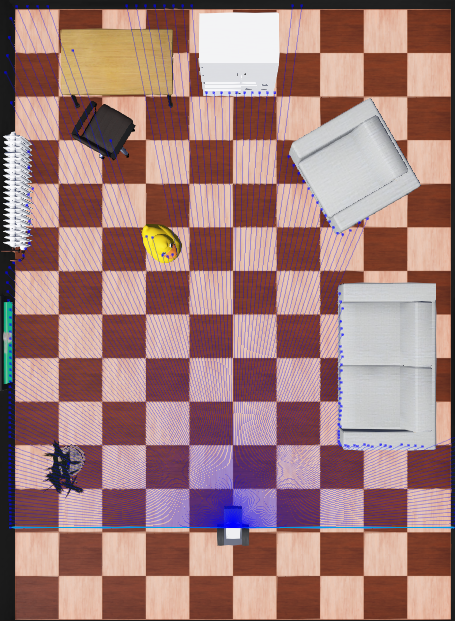
\includegraphics[width = 0.6\textwidth]{lidar_env.PNG}
            \caption{The simulation environment.}
            \label{fig:lidar_env}
        \end{subfigure}        
        \begin{subfigure}[b]{0.4\textwidth}
            \centering
            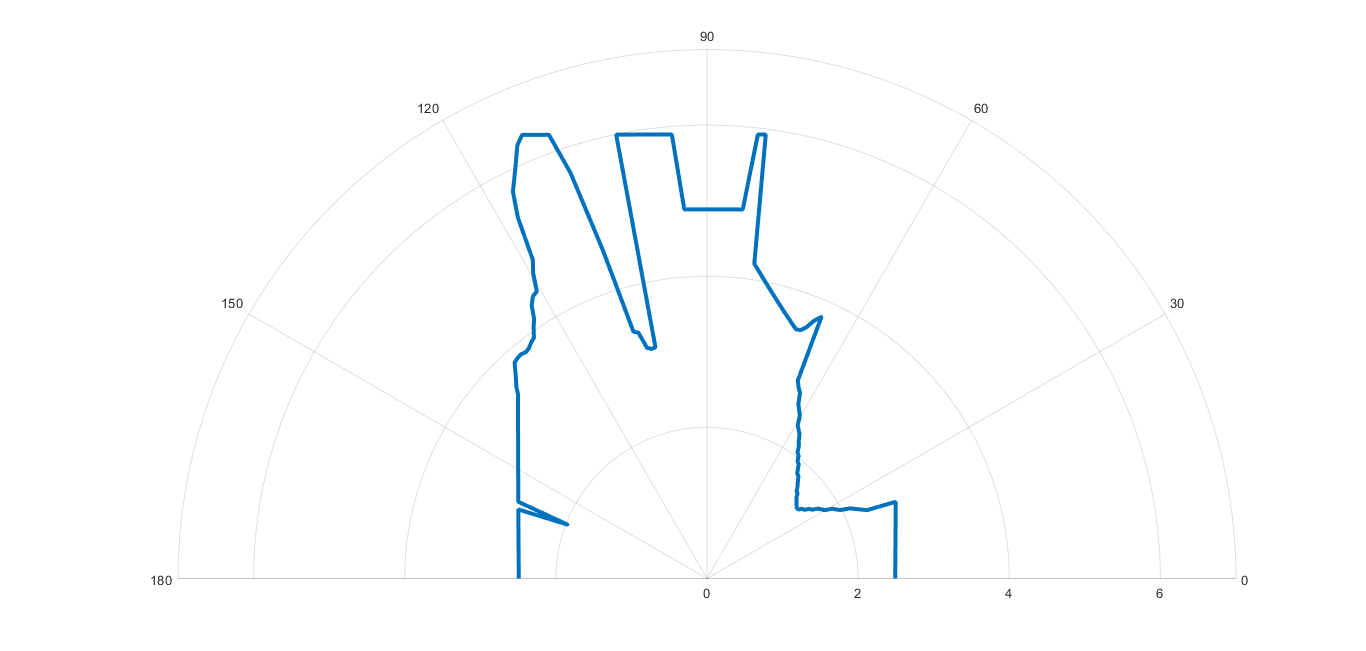
\includegraphics[width = 1.2\textwidth]{lidar_data.png}
            \caption{Polar plot of the distance sensor data.}
            \label{fig:lidar_data}
        \end{subfigure}
        \caption{Lidar sensor data in Webots Simulation.}
        \label{fig:lidar}
    \end{figure}

    \subsection{Defining map environment}
    Webots, offers a variety of objects below \emph{Proto Nodes}. These objects can be used to create a map environment. In this assignment, a map environment is created by adding typical living room objects to the \emph{Scene Tree}. The map environment is shown in Figure \ref{fig:map}.
    Alternatively different obstacles or landmarks can be placed in the simulation environment using \emph{Solid} nodes with \emph{boundingObjects}.  
    \begin{figure}[ht!]
        \centering
        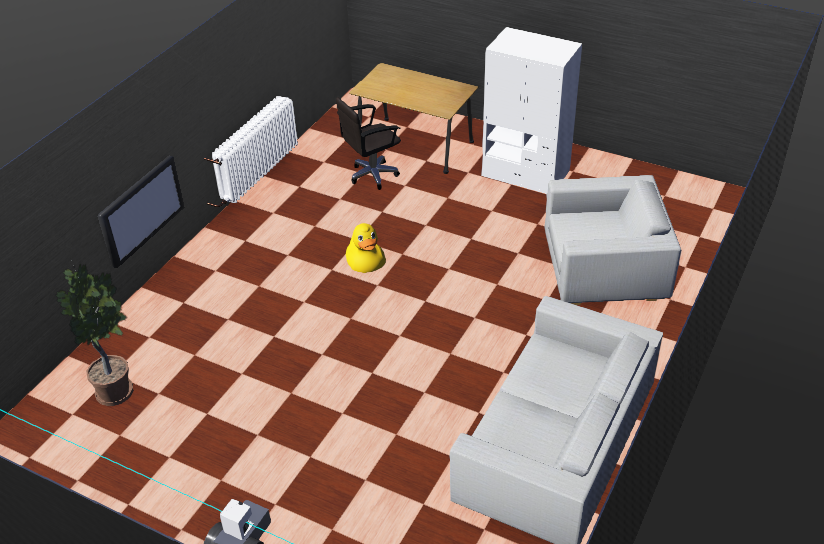
\includegraphics[width = 0.35\textwidth]{map.PNG}
        \caption{Map environment.}
        \label{fig:map}
    \end{figure}
    \subsection{Odometry Data}
    As mentioned before, differential drive robot includes two \emph{PositionalSensor}, these devices simulates encoder. Odometry data can be get from these sensors. In order to get the odometry data, sensors should be called using \emph{getDevice}, then enabled and finally the distance data can be obtained using \emph{getValue} method.
    Note that the odometry data is in radians, if the data is needed in meters, it should be converted by multiplying the data with the wheel radius. However, this calculation is only valid for linear motion. To compute the position of the robot from encoder data we
    need to take into account both the angular velocity and linear velocity of the robot using equations below and integrate them.
    \begin{align}
        v &= \frac{v_{left} + v_{right}}{2} \\
        w &= \frac{v_{left} - v_{right}}{d} \\
        \dot{\theta} &= w \\
        \dot{x} &= v \cos(\theta) \\
        \dot{y} &= v \sin(\theta) \\
    \end{align}
    Where $d$ is the distance between two wheels, $v_{left}$ and  $v_{right}$ are the linear velocities of the respective wheels.  \\
    In order to visualize odometry data, robot is moved in a square path with $1.5 \ m$ side length. The odometry data is saved to a txt file and plotted in MATLAB. 
    For comparison, the robot is equipped with a GPS sensor. The GPS sensor data is also saved to a txt file and added to same plot. The GPS and the odometry data is shown in Figure \ref{fig:odometry}.
    The odometry data is shown with blue '$*$', GPS data is shown in orange circles. Even without noise in the odometry data there are small discrapancies between the two data sets. This is due to numerical errors introduced from the odometry data calculations.
    A more detailed information on position sensors can be found in the \href{https://cyberbotics.com/doc/reference/positionsensor}{\emph{Webots Reference Manual} documentation}.
    \begin{figure}[ht!]
        \centering
        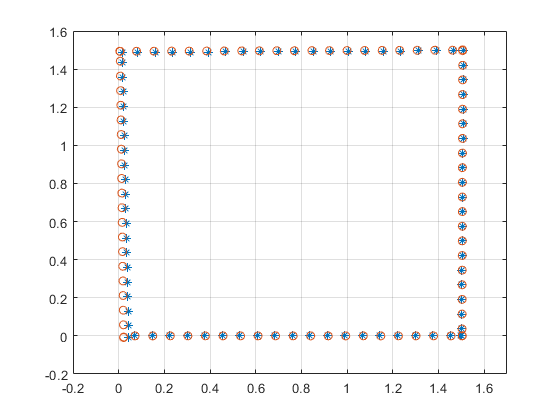
\includegraphics[width = 0.35\textwidth]{odometry_data.png}
        \caption{Odometry and GPS data.}
        \label{fig:odometry}
    \end{figure}
    

    \subsection{Camera Data}
    A \emph{Camera} node is added as a children node to the robot. Various aspects of the camera can be modified from the camera setups. Such as resolution, field of view, noise amd spherical distortion. When camera is enabled from the controller, the resulting image is displayed in 3D window.
    The camera pixel informations can be obtained using \emph{getImage} method. The image array is converted to RGB and saved to as a png file. The camera image is shown in Figure \ref{fig:camera}. A more detailed information on camera nodes can be found in the \href{https://cyberbotics.com/doc/reference/camera}{\emph{Webots Reference Manual} documentation}.
   
    \begin{figure}[ht!]
        \centering
        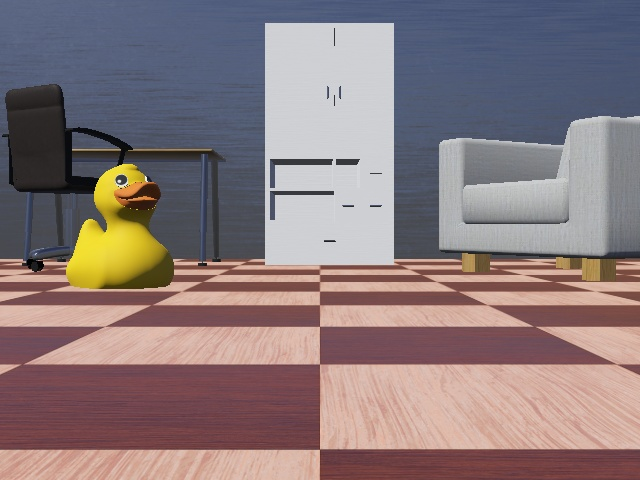
\includegraphics[width = 0.35\textwidth]{camera.jpg}
        \caption{Camera image.}
        \label{fig:camera}
    \end{figure}
    \subsection{Simulating sensor noise}
    The lidar, position sensor and camera nodes offer noise parameters. These parameters can be used to simulate noise in the sensor data. 
    All the sensors are modified to have noise parameters. In the Figure \ref{fig:lidar-noise}, the noisy lidar data is given in comparison with the previous noiseless data in Figure \ref{fig:lidar_data}. The noise is set to $0.2$.
    The noisy data is shown in orange and noiseless data is shown in blue. 
    \begin{figure}[ht!]
        \centering
        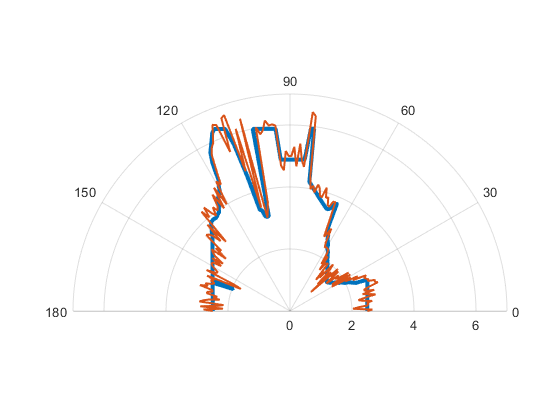
\includegraphics[width = 0.35\textwidth]{noisy_lidar.png}
        \caption{Noisy lidar data compared to noiseless data.}
        \label{fig:lidar-noise}
    \end{figure}
    \\
    \noindent The odometry data from noisy position sensor is shown in Figure \ref{fig:odometry-noise}. The noise is set to $0.2$ for the position sensor on the each wheel. The data is collected in a square path with $1.5 \ m$ side length and compared with noiseless GPS data as the ground truth.
    The noisy odometry data is shown in blue and noiseless GPS data is shown in orange. 
    There is a significant difference between the odometry and GPS data due to noise.
    \begin{figure}[ht!]
        \centering
        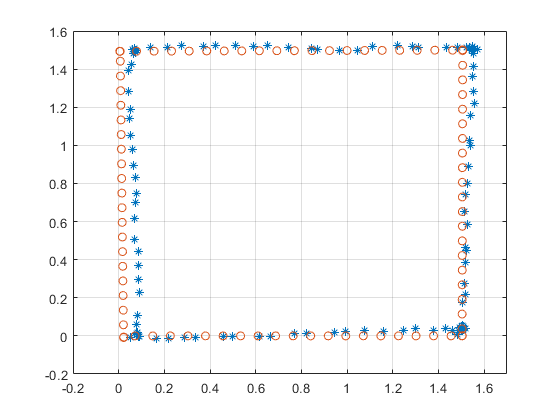
\includegraphics[width = 0.4\textwidth]{noisy_encoder.png}
        \caption{Noisy odometry data compared to ground truth GPS data.}
        \label{fig:odometry-noise}
    \end{figure}
    \\
    \noindent The camera noise is set to $0.2$ and the resulting image is shown in Figure \ref{fig:camera-noise}. The effect of noise on the image pixels is visible in the image when compared to the noiseless image in Figure \ref{fig:camera}.
    \begin{figure}[ht!]
        \centering
        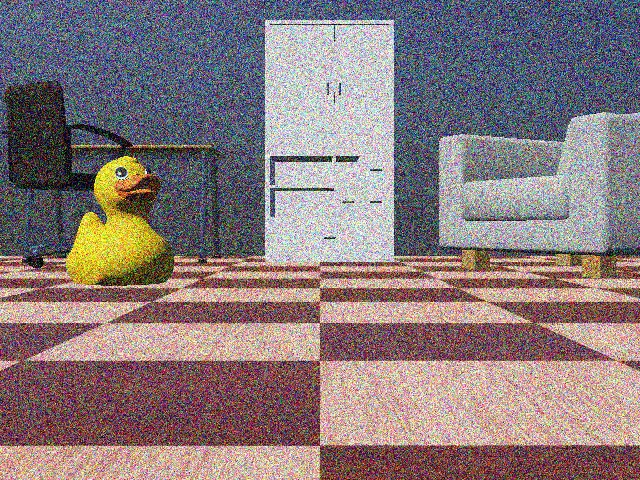
\includegraphics[width = 0.4\textwidth]{noisy_camera.jpg}
        \caption{Noisy camera image.}
        \label{fig:camera-noise}
    \end{figure}

    \section{Robot Following Task}
    In the following task, camera sensor is used for identifying and tracking the leading robot. The leading robot is fitted with a green spherical solid at the back bumper. 
    The controller of the robot behind the leading robot takes camera image and extracts the contour of the green ball by using OpenCV library. The center of the green ball is calculated and 
    the controller uses a proportional controller to steer the differential drive to keep the ball in the center of the image. The tracking distance is set to $0.65 \ m$. To keep the distance stable,
    the controller uses another proportional controller to set the linear velocity of the robot. The radius of the ball is used as a measure of distance to the leading robot. The distance between two robots is shown in Figure \ref{fig:distance}.
    \begin{figure}[ht]
        \centering
        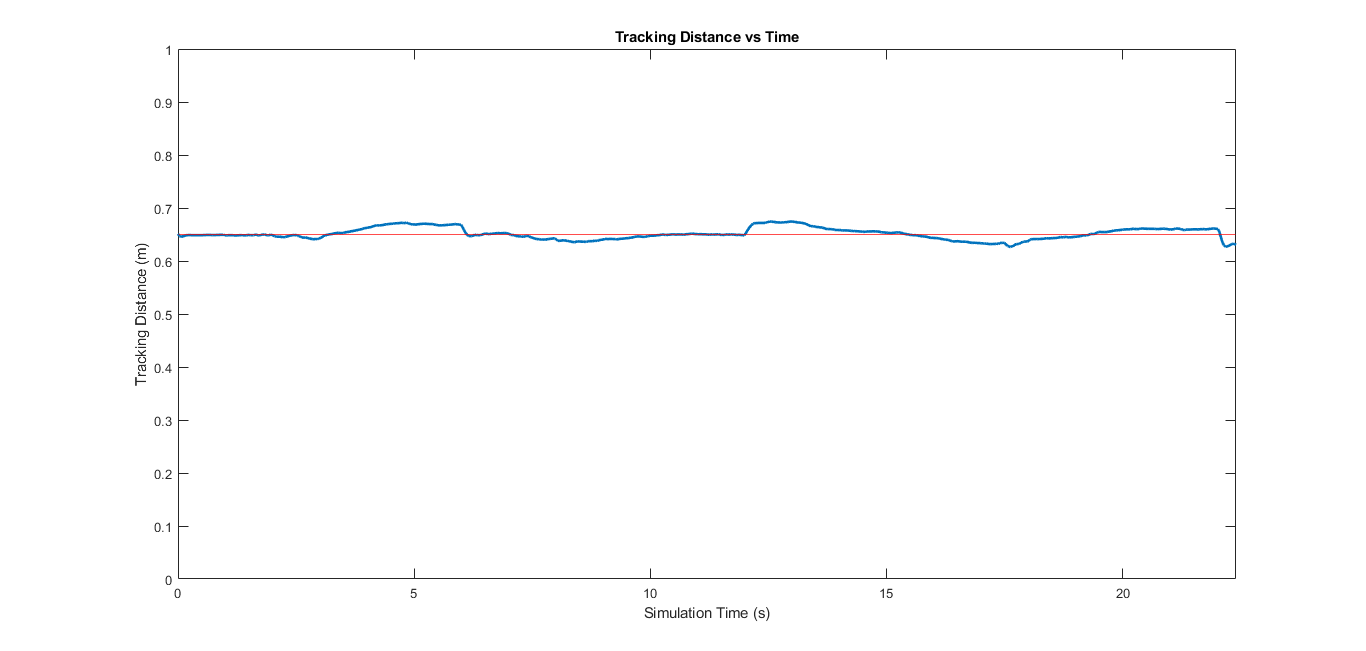
\includegraphics[width = 0.6\textwidth]{track_distance.png}
        \caption{Tracking Distance vs Time.}
        \label{fig:distance}
    \end{figure}
    \\
    \noindent The controller performs following task with a bounded tracking distance fluctuating between $0.6 \ m$ and $0.7 \ m$. A sample video of the robot following task is available \href{https://www.youtube.com/watch?v=KW6KgzZL-Is}{online}.

    \end{document}
